\section{The analytic solution}
An analytic solution to this problem with variable viscosity is only possible for special forms of \(\nu(z)\). For example if \(\nu(z)\) varies exponentially with height
\begin{equation}
    \nu(z) = \nu_0 \exp\left(\beta{z}\right),
\end{equation}, an analytic solution exists. 
This can be seen by using the anstaz:
\begin{equation}
    \begin{cases}
        \tilde u'(z) = -A(z)u_0  \exp\left({-\frac{z}{\delta}}\right) \cos\left(\frac{z}{\delta}\right), \\
        \tilde v(z) = A(z)u_0  \exp\left({-\frac{z}{\delta}}\right) \sin\left(\frac{z}{\delta}\right),
    \end{cases}
\end{equation}
for an arbitraru slowly varying function \(A(z)\). Inserting this into the original equations gives a differential equation for \(A(z)\) which can be solved analytically. The solution is given by
\begin{equation}
A(z) = 
\exp\!\left( -\frac{f\, \delta}{2\nu_0 \beta} \right)
\exp\!\left( 
\frac{z}{\delta}
+ \frac{f\, \delta}{2\nu_0 \beta} e^{-\beta z}
\right).
\end{equation}
Which gives the full solution
\begin{equation}
    \begin{cases}
        \tilde u'(z) = -u_0  \exp\!\left[  \frac{f\, \delta}{2\nu_0 \beta} \left(e^{-\beta z}-1\right)\right]  \cos\left(\frac{z}{\delta}\right), \\
        \tilde v(z) = -_0  \exp\!\left[  \frac{f\, \delta}{2\nu_0 \beta} \left(e^{-\beta z}-1\right)\right]  \sin\left(\frac{z}{\delta}\right).
    \end{cases}
\end{equation}

\begin{figure}[H]
    \centering    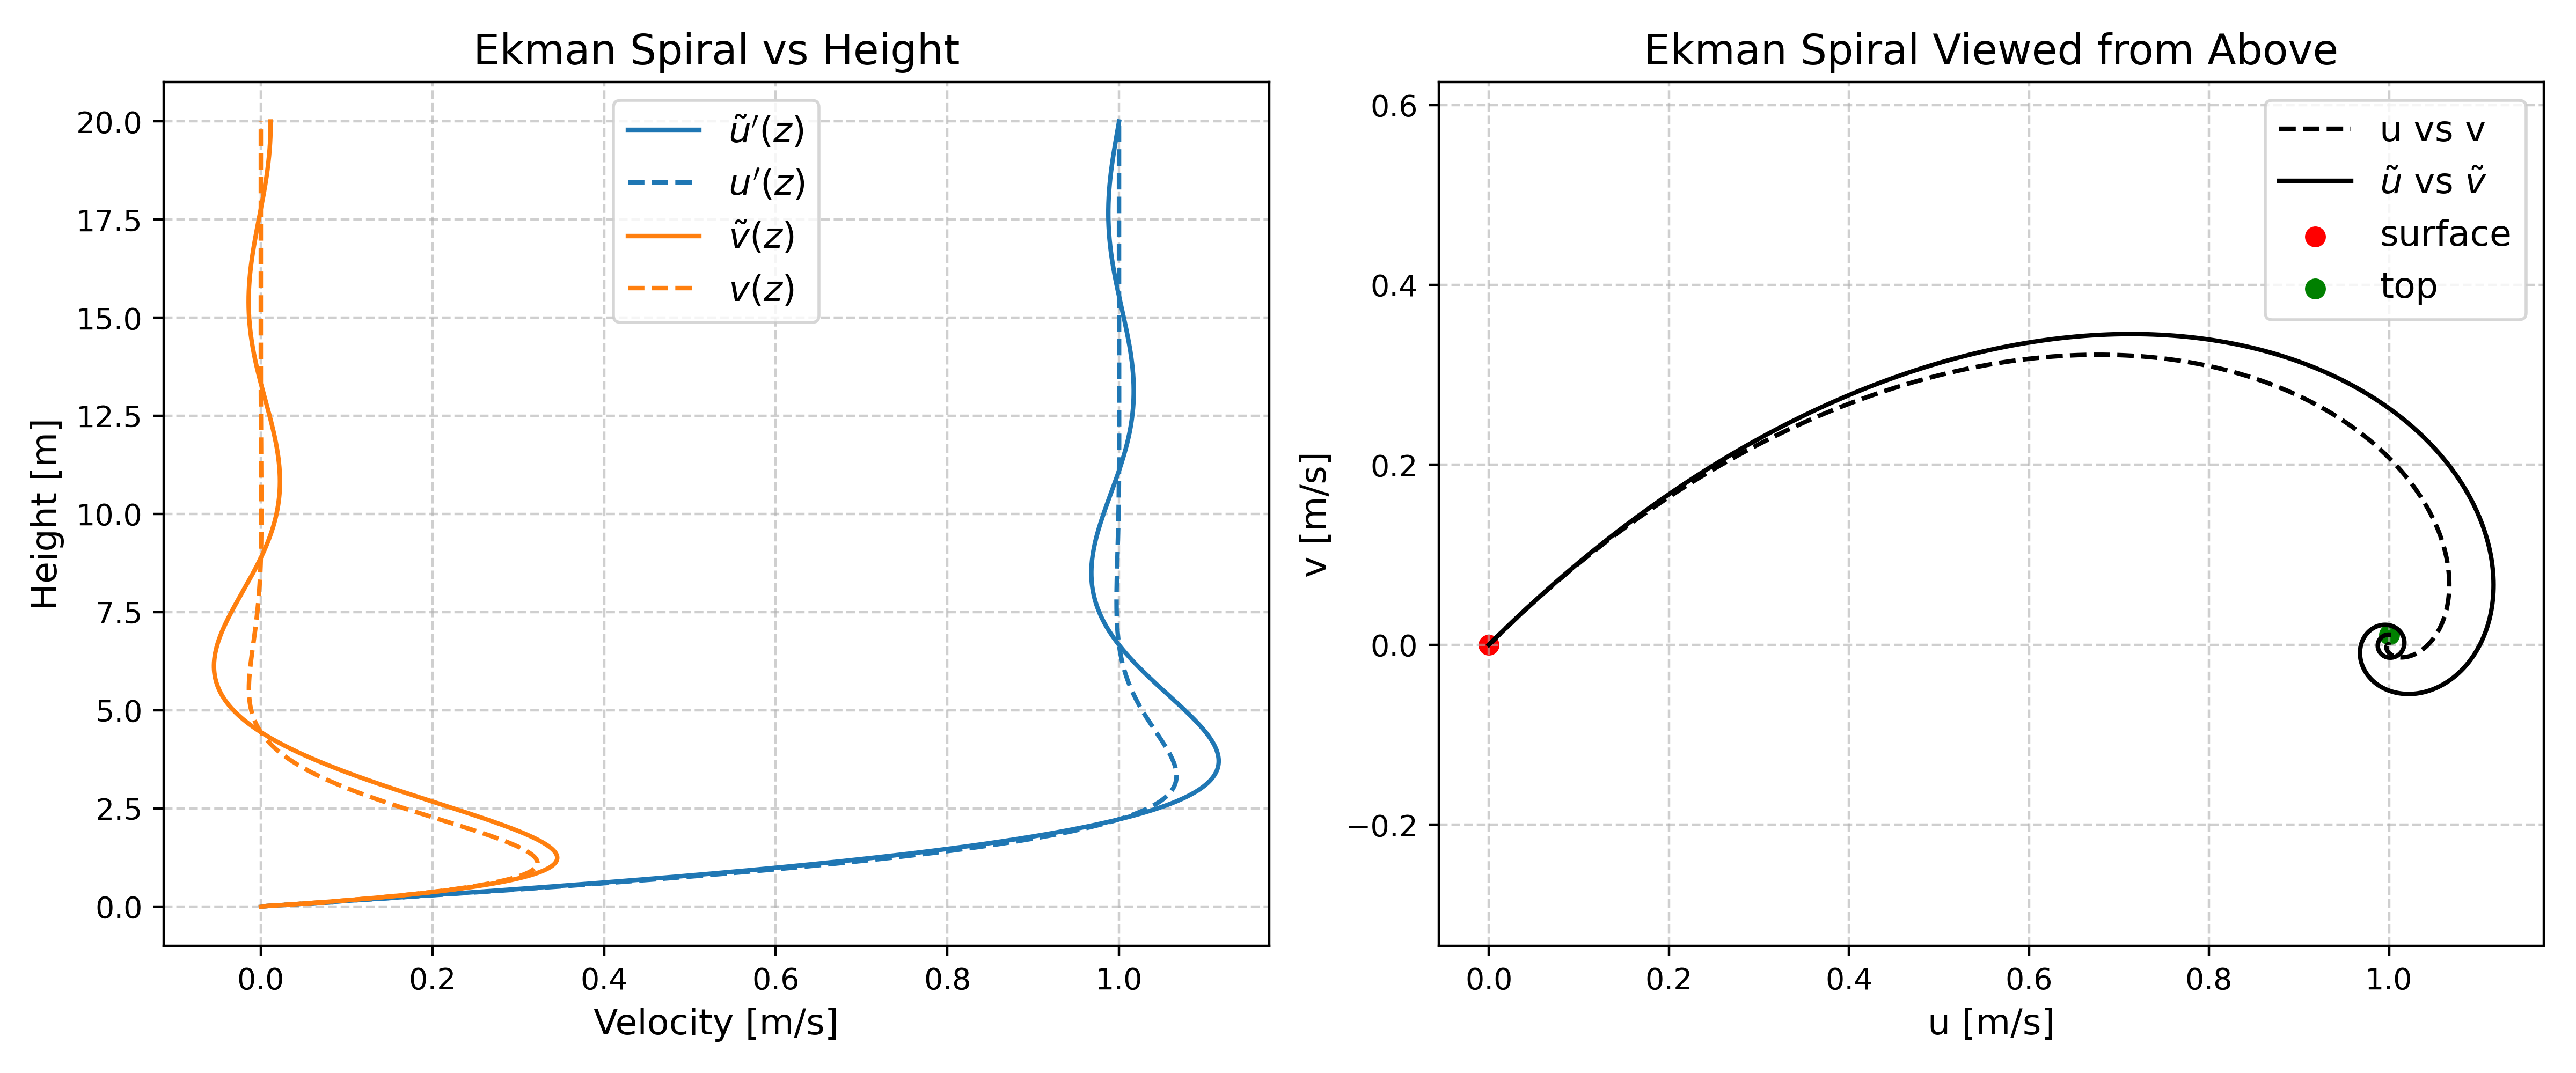
\includegraphics[width=0.9\textwidth]{Figures/analytic_b=0.15.png}
    \caption{This figure shows the analytic solution for an exponentially increasing viscosity with \(\beta=0.15\,\text{m}^{-1}\).}
    \label{fig:analytic}
\end{figure}
